\documentclass[11pt]{article}

% ── Packages ──────────────────────────────────────────────────────────
\usepackage{amsmath,amsthm,amssymb}
\usepackage[round]{natbib}
\usepackage{booktabs}
\usepackage{graphicx}
\usepackage[colorlinks=true,citecolor=blue,linkcolor=blue,urlcolor=blue]{hyperref}
\usepackage[margin=1in]{geometry}
\usepackage{setspace}
\onehalfspacing

% ── Theorem environments ─────────────────────────────────────────────
\newtheorem{assumption}{Assumption}
\newtheorem{proposition}{Proposition}
\newtheorem{corollary}{Corollary}
\newtheorem{definition}{Definition}
\newtheorem{remark}{Remark}

% ── Title ─────────────────────────────────────────────────────────────
\title{Beyond Bond-Like Human Capital:\\
A Beta-Adjusted Framework for Lifecycle Portfolio Choice}
\author{Engineer Investor\thanks{%
Corresponding author. Email: \texttt{egr.investor@gmail.com}.
Software and replication code available at
\url{https://github.com/engineerinvestor/lifecycle-allocation}.}}
\date{\today}

\begin{document}
\maketitle

% ══════════════════════════════════════════════════════════════════════
% Abstract
% ══════════════════════════════════════════════════════════════════════
\begin{abstract}
Standard lifecycle portfolio models treat human capital as a risk-free,
bond-like asset, leading to aggressive equity recommendations for young
workers. This assumption fails systematically for employees in technology,
startups, finance, and commission-based roles, where compensation is
substantially correlated with equity markets through restricted stock units
(RSUs), equity grants, and cyclical layoff exposure. We propose a
parsimonious extension to the \citet{choi2025} lifecycle framework: a human
capital beta parameter, $\beta_H \in [0,1]$, that decomposes human capital
into bond-like and equity-like components. The modified allocation rule,
$\alpha = \alpha^{*}\!\bigl(1 + (1-\beta_H)\,H/W\bigr)$, nests the
standard model ($\beta_H = 0$) and produces materially different
recommendations for workers with equity-like income. For a 30-year-old
technology worker with RSU-heavy compensation ($\beta_H = 0.60$), the
framework recommends approximately 30 percentage points less equity than
the standard model. We calibrate industry-specific betas from labor
economics literature and implement the framework in an open-source Python
package \citep{lifecycle_allocation}.

\medskip
\noindent\textbf{JEL Classification:} G11, G51, J31, D15\\
\textbf{Keywords:} lifecycle portfolio choice, human capital, labor income
risk, asset allocation, risk-adjusted human capital
\end{abstract}

\newpage

% ══════════════════════════════════════════════════════════════════════
\section{Introduction}\label{sec:intro}
% ══════════════════════════════════════════════════════════════════════

A central insight of lifecycle portfolio theory is that young investors
should hold more equity than old investors because their human capital, the
present value of future earnings, functions as an implicit bond position
\citep{merton1969, bodie1992}. The logic is compelling: a government
employee with a stable, inflation-indexed salary effectively owns a large
bond, and her financial portfolio should tilt toward equities to diversify
her total wealth.

This reasoning, however, rests on an assumption that is increasingly at
odds with modern labor markets. For a software engineer at a publicly
traded technology company, 30 to 50 percent of total compensation may
arrive as restricted stock units (RSUs) that vest over multiple years. For
a startup founder, virtually all compensation is tied to the equity value
of a single, undiversified firm. For a commission-based financial advisor,
income fluctuates with asset prices and trading volumes. In each of these
cases, human capital is not bond-like; it is equity-like, correlated with
the very market risk that the standard model tells the investor to load up
on.

The consequences of ignoring this correlation are not merely theoretical.
Consider a 30-year-old technology worker earning \$200{,}000 per year with
\$100{,}000 in savings. The standard lifecycle model, treating her human
capital as a riskless asset, might recommend 95 percent or more in equities.
Yet her RSU holdings already expose her to significant market risk,
particularly concentrated in a single sector. A market downturn that
reduces her portfolio value is likely to coincide with RSU depreciation,
hiring freezes, or layoffs, amplifying the shock to her total wealth.

This paper proposes a simple, tractable extension to the lifecycle
framework of \citet{choi2025}. We introduce a single parameter,
$\beta_H \in [0,1]$, representing the fraction of human capital that is
equity-like. The modified allocation formula becomes
\begin{equation}\label{eq:main}
  \alpha = \alpha^{*}\!\Bigl(1 + (1 - \beta_H)\,\frac{H}{W}\Bigr),
\end{equation}
where $\alpha^{*}$ is the Merton baseline risky share, $H$ is the present
value of human capital, and $W$ is investable financial wealth. When
$\beta_H = 0$, the formula reduces to the standard model. When
$\beta_H > 0$, the equity-like portion of human capital is excluded from
the diversification adjustment, producing a lower, more prudent equity
recommendation.

Our contribution is threefold. First, we provide a formal derivation
showing that the beta-adjusted formula arises naturally from a CRRA utility
maximization problem with correlated human capital. Second, we calibrate
industry-specific beta values using data from labor economics, drawing on
\citet{davis2000}, \citet{benzoni2007}, and compensation structure
analysis. Third, we implement the framework in an open-source Python
package, \texttt{lifecycle-allocation} \citep{lifecycle_allocation}, making
it immediately available to researchers, financial advisors, and
robo-advisory platforms.

The remainder of the paper is organized as follows. Section~\ref{sec:lit}
reviews the related literature. Section~\ref{sec:model} develops the
beta-adjusted model and states its key properties.
Section~\ref{sec:calibration} discusses the calibration of industry-specific
betas. Section~\ref{sec:results} presents comparative statics and case
studies. Section~\ref{sec:discussion} discusses limitations and extensions.
Section~\ref{sec:conclusion} concludes.


% ══════════════════════════════════════════════════════════════════════
\section{Literature Review}\label{sec:lit}
% ══════════════════════════════════════════════════════════════════════

The theoretical foundations of lifecycle portfolio choice trace back to
\citet{merton1969, merton1971}, who derived the continuous-time optimal
consumption and portfolio rules for an investor with constant relative risk
aversion (CRRA) utility. In the absence of labor income, the optimal equity
allocation is the well-known Merton ratio:
\begin{equation}\label{eq:merton}
  \alpha^{*} = \frac{\mu - r}{\gamma \sigma^2},
\end{equation}
where $\mu$ is the expected equity return, $r$ is the risk-free rate,
$\gamma$ is the coefficient of relative risk aversion, and $\sigma$ is
equity return volatility. This allocation is constant over time and
independent of wealth, a consequence of the CRRA assumption.

\citet{bodie1992} introduced labor supply flexibility into the lifecycle
model, showing that the ability to adjust hours worked functions as an
implicit form of insurance. Their key insight was that human capital, the
capitalized value of future wages, acts as a bond-like asset in the
investor's total portfolio. Because young workers have large human capital
relative to financial wealth, they should hold a higher equity share in
their financial portfolio to achieve the optimal allocation across total
wealth. This result provided the first rigorous justification for the
conventional wisdom that young investors should favor equities.

\citet{viceira2001} extended the analysis to settings with nontradable
labor income, deriving optimal portfolio rules in a partial equilibrium
framework. His model allowed for stochastic income but maintained the
assumption that income shocks are largely uncorrelated with asset returns.
The resulting optimal strategy still features a declining equity allocation
with age, though the magnitude depends on income volatility and the degree
of market incompleteness.

The computational lifecycle literature, exemplified by
\citet{cocco2005}, solved the full dynamic programming problem
numerically. Their calibration, which matched income processes to Panel
Study of Income Dynamics (PSID) data by education group, confirmed the
qualitative predictions of the analytical models: young households should
hold nearly 100 percent equities, declining gradually with age. However,
their baseline calibration assumed zero correlation between permanent income
shocks and equity returns, a parameter choice that is critical for our
purposes.

\citet{benzoni2007} challenged the zero-correlation assumption directly.
Using a model in which labor income and stock dividends are cointegrated,
they showed that the long-run correlation between human capital and equity
returns can be substantial, even when short-run correlations are low. Their
results imply that young workers, whose human capital is most exposed to
long-run cointegration effects, should hold less equity than the standard
model recommends. The cointegration channel is particularly relevant for
workers in cyclical industries where long-run income growth tracks
aggregate productivity.

On the empirical side, \citet{davis2000} estimated occupation-level income
betas by regressing income growth on asset returns across a panel of
industries. They found significant heterogeneity: income in goods-producing
sectors, finance, and insurance exhibited much higher market betas than
income in government, education, and healthcare. Their work provides the
most direct empirical basis for calibrating industry-specific human capital
betas.

\citet{jagannathan1996} developed a conditional CAPM framework in which
human capital is a priced factor. Their approach treats aggregate labor
income as a proxy for the return on human capital, providing a
macroeconomic perspective on the same phenomenon we address at the
individual level. \citet{campbell1996} further explored the relationship
between labor income risk and the cross-section of expected returns,
emphasizing that the riskiness of human capital varies systematically with
occupation and industry.

The strategic asset allocation literature, surveyed comprehensively by
\citet{campbell2002}, integrates these insights into practical portfolio
advice. Campbell and Viceira emphasized the importance of the
investor's labor income profile in determining the optimal equity share,
noting that ``safe'' labor income (government employment, tenured academic
positions) supports a higher equity allocation than ``risky'' labor income
(entrepreneurship, commission-based sales).

More recently, \citet{choi2025} developed an approximate closed-form
solution to the lifecycle portfolio choice problem that is both practically
useful and theoretically grounded. Their framework, which our model extends,
produces the allocation rule $\alpha = \alpha^{*}(1 + H/W)$, where the
human capital adjustment captures the implicit bond position. The
\citet{choi2025} model is notable for its simplicity and tractability,
making it an ideal platform for the kind of parsimonious extension we
propose.

Several related contributions deserve mention. \citet{fama1993} established
the multi-factor framework that motivates thinking about labor income as
exposure to systematic risk factors. \citet{heaton2000} demonstrated that
entrepreneurial risk, a form of concentrated human capital, has
first-order effects on portfolio choice and asset prices, with
entrepreneurs rationally holding less equity in their financial portfolios.

Despite this rich literature, a gap persists between the theoretical
recognition that human capital risk matters and the practical tools
available to incorporate it. Existing models either ignore the correlation
between human capital and equity returns (the standard lifecycle approach)
or require complex numerical solutions that are difficult to implement and
calibrate (the Benzoni, Collin-Dufresne, and Goldstein approach). Our
contribution fills this gap by proposing a single-parameter adjustment that
nests the standard model, admits a closed-form solution, and can be
calibrated from readily available data on compensation structure and
industry risk.


% ══════════════════════════════════════════════════════════════════════
\section{Model}\label{sec:model}
% ══════════════════════════════════════════════════════════════════════

\subsection{The Standard Lifecycle Model}\label{sec:standard}

We begin by recapping the standard lifecycle allocation framework of
\citet{choi2025}. An investor of age $t$ has financial wealth $W_t > 0$
and human capital
\begin{equation}\label{eq:hc}
  H_t = \sum_{s=t+1}^{T_{\max}} \frac{\mathbb{E}[CF_s] \cdot S(t,s)}{D(t,s)},
\end{equation}
where $CF_s$ denotes the cash flow at age $s$ (income before retirement,
benefits after retirement), $S(t,s)$ is the conditional survival probability
from age $t$ to age $s$, and $D(t,s)$ is the discount factor.

Total wealth is $\Omega_t = W_t + H_t$. The investor maximizes CRRA
utility over terminal wealth with risk aversion $\gamma > 0$. In the
standard model, human capital is assumed to be riskless (perfectly
correlated with the bond), so the optimal equity share in total wealth is
the Merton ratio $\alpha^{*}$ from equation~\eqref{eq:merton}. Translating
this into a recommendation for the financial portfolio yields
\begin{equation}\label{eq:standard}
  \alpha_t = \alpha^{*}\!\left(1 + \frac{H_t}{W_t}\right),
\end{equation}
clamped to $[0,1]$ (or $[0, L_{\max}]$ if leverage is permitted). The
intuition is straightforward: human capital is a bond, so the financial
portfolio must overweight equity to achieve the target allocation across
total wealth.

\subsection{The Beta-Adjusted Model}\label{sec:beta}

We now relax the assumption that human capital is entirely bond-like. Let
$\beta_H \in [0,1]$ denote the fraction of human capital whose returns are
correlated with the equity market. We decompose:
\begin{equation}\label{eq:decompose}
  H_t = H_t^{\text{bond}} + H_t^{\text{equity}},
  \quad\text{where}\quad
  H_t^{\text{equity}} = \beta_H \cdot H_t
  \quad\text{and}\quad
  H_t^{\text{bond}} = (1 - \beta_H)\cdot H_t.
\end{equation}

The bond-like component $H_t^{\text{bond}}$ continues to function as an
implicit fixed-income position; it diversifies the financial portfolio and
calls for a higher equity share. The equity-like component
$H_t^{\text{equity}}$, however, is already exposed to market risk. From a
portfolio perspective, it behaves like an implicit equity position that the
investor cannot sell or rebalance.

Only the bond-like portion provides a diversification benefit in the
financial portfolio. The modified allocation rule is therefore
\begin{equation}\label{eq:beta_adjusted}
  \alpha_t = \alpha^{*}\!\left(1 + (1-\beta_H)\,\frac{H_t}{W_t}\right),
\end{equation}
clamped to $[0,1]$ or $[0, L_{\max}]$. This formula nests the standard
model: setting $\beta_H = 0$ recovers equation~\eqref{eq:standard}.

\begin{definition}[Human Capital Beta]\label{def:beta}
The \emph{human capital beta}, $\beta_H \in [0,1]$, is the fraction of
the present value of future earnings whose returns are correlated with
the equity market. A beta of zero corresponds to fully bond-like human
capital (e.g., government employment with inflation-indexed pension). A
beta of one corresponds to fully equity-like human capital (e.g., a
startup founder compensated entirely in company equity).
\end{definition}

\subsection{Derivation}\label{sec:derivation}

We provide a sketch of the formal derivation. Consider an investor
maximizing expected CRRA utility:
\begin{equation}
  \max_{\alpha}\; \mathbb{E}\!\left[\frac{(\Omega_T)^{1-\gamma}}{1-\gamma}\right],
\end{equation}
where $\Omega_T$ is terminal total wealth and $\gamma > 1$. Total wealth
at each period evolves as
\begin{equation}
  \Omega_{t+1} = \bigl[\alpha_t R_e + (1-\alpha_t) R_f\bigr]\,W_t + \tilde{H}_{t+1},
\end{equation}
where $R_e$ and $R_f$ are gross equity and risk-free returns, $W_t$ is
financial wealth, and $\tilde{H}_{t+1}$ is the stochastic next-period
value of human capital.

\begin{assumption}\label{as:beta}
Human capital generates cash flows with market correlation $\beta_H$.
Specifically, the return on the ``human capital portfolio'' can be
decomposed as
\begin{equation}
  \tilde{r}_H = \beta_H \tilde{r}_e + (1-\beta_H)\,r_f + \tilde{\varepsilon},
\end{equation}
where $\tilde{\varepsilon}$ is idiosyncratic risk uncorrelated with
$\tilde{r}_e$ and diversified away in the human capital PV calculation.
\end{assumption}

Under Assumption~\ref{as:beta}, the investor's total equity exposure is
\begin{equation}
  \text{Equity exposure} = \alpha_t W_t + \beta_H H_t.
\end{equation}
The first term is the explicit equity position in the financial portfolio;
the second is the implicit equity exposure embedded in human capital.

The optimal total equity share in total wealth is still the Merton ratio
$\alpha^{*}$. Setting total equity exposure equal to the target:
\begin{equation}
  \alpha_t W_t + \beta_H H_t = \alpha^{*}(W_t + H_t).
\end{equation}
Solving for the financial portfolio equity share:
\begin{align}
  \alpha_t &= \alpha^{*}\,\frac{W_t + H_t}{W_t} - \beta_H\,\frac{H_t}{W_t} \nonumber\\
           &= \alpha^{*}\!\left(1 + \frac{H_t}{W_t}\right) - \beta_H\,\frac{H_t}{W_t} \nonumber\\
           &= \alpha^{*} + (\alpha^{*} - \beta_H)\,\frac{H_t}{W_t}. \label{eq:derived_alt}
\end{align}

When $\beta_H = 0$, this reduces to the standard formula~\eqref{eq:standard}.
We can equivalently rewrite equation~\eqref{eq:derived_alt} as
\begin{equation}
  \alpha_t = \alpha^{*}\!\left(1 + \frac{H_t}{W_t}\right) - \beta_H\,\frac{H_t}{W_t}.
\end{equation}

For the special case where we set
$\alpha_t = \alpha^{*}\!\bigl(1 + (1-\beta_H)\,H_t/W_t\bigr)$, this is
equivalent to
\begin{equation}
  \alpha_t = \alpha^{*} + \alpha^{*}(1-\beta_H)\,\frac{H_t}{W_t},
\end{equation}
which differs from~\eqref{eq:derived_alt} by a term
$(\alpha^{*} - 1)\,\beta_H\,H_t/W_t$. This approximation is exact when
$\alpha^{*} = 1$ and is tight whenever $\alpha^{*}$ is close to one or
$\beta_H$ is small, conditions that hold for a wide range of empirically
relevant parameterizations. We adopt the simpler
form~\eqref{eq:beta_adjusted} for tractability and note that the
implementation in \texttt{lifecycle-allocation} uses this formula.

\begin{remark}\label{rem:exact}
The exact decomposition in equation~\eqref{eq:derived_alt} can be
implemented as an alternative mode in the software. For typical
calibrations ($\alpha^{*} \in [0.5, 1.5]$, $\beta_H \in [0, 0.6]$),
the two formulas differ by at most a few percentage points.
\end{remark}

\subsection{Embedded Options Perspective}\label{sec:options}

The parameter $\beta_H$ captures the average equity exposure of human
capital, but the underlying compensation structure often contains
option-like features that create nonlinear risk exposures.

\textbf{RSU vesting as call options.} Restricted stock units vest
over a multi-year schedule, typically four years with a one-year cliff.
The unvested portion is analogous to a portfolio of call options on the
employer's stock: the employee benefits from price appreciation but faces
forfeiture risk upon termination. Because termination probability increases
during market downturns (through layoffs and restructuring), the
effective delta of these ``options'' is higher than for exchange-traded
calls.

\textbf{Layoff risk as a short put.} An employee's continued
employment can be viewed as a short put option on the employer's business
prospects. In normal times, the option expires worthless, and the employee
collects her wages. During severe downturns, the ``option'' is exercised:
the employee is laid off, losing both current income and unvested equity
compensation. This asymmetry means that the downside correlation between
human capital and equity markets exceeds the average correlation.

\textbf{Career mobility as a real option.} Workers with transferable
skills hold a real option to switch industries, effectively an option
to reduce $\beta_H$ at the cost of potential income reduction. This
option has value and partially mitigates the risk of equity-like human
capital. Industries with strong demand for specialized skills (e.g.,
software engineering, quantitative finance) provide more valuable mobility
options.

\textbf{Non-competes and golden handcuffs.} Contractual restrictions
such as non-compete agreements and deferred compensation structures reduce
the value of the career mobility option, effectively increasing the
employee's lock-in to the current employer's risk profile.

These option-like features suggest that a single scalar $\beta_H$ is a
first-order approximation to a richer risk structure. Nevertheless, for
practical portfolio advice, the scalar parameterization captures the most
important dimension of variation across industries and compensation types.

\subsection{Formal Properties}\label{sec:properties}

\begin{proposition}[Monotonicity in $\beta_H$]\label{prop:mono}
For fixed $W > 0$, $H \geq 0$, and $\gamma > 0$, the recommended equity
allocation $\alpha(\beta_H)$ is monotonically non-increasing in $\beta_H$.
\end{proposition}

\begin{proof}
From equation~\eqref{eq:beta_adjusted},
\begin{equation}
  \frac{\partial \alpha}{\partial \beta_H}
  = -\alpha^{*}\,\frac{H}{W}.
\end{equation}
Since $\alpha^{*} \geq 0$ (the equity premium is non-negative for any
reasonable calibration) and $H/W \geq 0$, we have
$\partial\alpha / \partial\beta_H \leq 0$, establishing
non-increasing monotonicity.
\end{proof}

\begin{corollary}[Equity-Like Human Capital Irrelevance]\label{cor:beta1}
When $\beta_H = 1$, the allocation reduces to
$\alpha = \alpha^{*}$, independent of $H$.
\end{corollary}

\begin{proof}
Substituting $\beta_H = 1$ into equation~\eqref{eq:beta_adjusted}:
\begin{equation}
  \alpha = \alpha^{*}\!\left(1 + (1-1)\,\frac{H}{W}\right)
         = \alpha^{*}\!\left(1 + 0\right)
         = \alpha^{*}.
\end{equation}
The human capital term vanishes entirely.
\end{proof}

The intuition for Corollary~\ref{cor:beta1} is clear: when human capital
is perfectly correlated with the equity market, it provides no
diversification benefit whatsoever. The investor's total equity exposure
from human capital alone already exceeds or matches what the optimal
portfolio requires, so the financial portfolio should not add further
equity exposure on account of human capital.


% ══════════════════════════════════════════════════════════════════════
\section{Calibration}\label{sec:calibration}
% ══════════════════════════════════════════════════════════════════════

Calibrating $\beta_H$ requires estimating the correlation between an
individual's income stream and equity market returns. We draw on three
sources: the occupation-level income regressions of \citet{davis2000}, the
cointegration estimates of \citet{benzoni2007}, and a compensation
structure analysis that accounts for the growing prevalence of equity-based
pay in technology and finance.

\citet{davis2000} regressed real income growth on asset returns across 62
occupations and industries. Their estimates reveal substantial
heterogeneity. Government and education workers show near-zero income
betas, consistent with the stable, contractually determined nature of
public-sector pay. Goods-producing industries (manufacturing, construction,
mining) exhibit moderate betas in the range of 0.20 to 0.50, reflecting
cyclical sensitivity. Finance and insurance show among the highest betas,
driven by bonus structures, commission income, and employment cyclicality.

\citet{benzoni2007} estimated the long-run cointegration relationship
between labor income and stock market dividends. Their key finding is that
the long-run beta of human capital is substantially higher than short-run
income-return correlations suggest, particularly for young workers with
long remaining careers. This implies that calibrations based solely on
contemporaneous income-return regressions may understate the true equity
exposure of human capital.

Our compensation structure analysis supplements these econometric estimates
with information about the form of compensation. An employee receiving 40
percent of total compensation in employer RSUs has a direct equity
exposure that is captured by $\beta_H$ but would not appear in aggregate
income regressions (which typically measure cash compensation). We
therefore adjust the econometric betas upward for industries where
equity-based compensation is prevalent.

Table~\ref{tab:betas} presents our calibrated industry betas, along with
the primary rationale for each estimate. The values range from 0.00 for
government and tenured education (fully bond-like) to 0.85 for
equity-heavy startup employees (nearly fully equity-like).

\begin{table}[ht]
\centering
\caption{Calibrated Industry Human Capital Betas}\label{tab:betas}
\smallskip
\begin{tabular}{@{}llp{6cm}@{}}
\toprule
\textbf{Industry / Role} & $\boldsymbol{\beta_H}$ & \textbf{Rationale} \\
\midrule
Government                & 0.00 & Inflation-indexed salary, defined benefit pension \\
Education (tenured)       & 0.00 & Tenure protection, stable public funding \\
Healthcare                & 0.10 & Demand inelastic, some reimbursement cyclicality \\
Utilities                 & 0.10 & Regulated returns, stable demand \\
Consumer staples          & 0.15 & Moderate cyclicality, low equity comp share \\
Education (non-tenured)   & 0.20 & At-will employment, enrollment sensitivity \\
Manufacturing             & 0.25 & Cyclical demand, layoff exposure \\
Professional services     & 0.30 & Moderate cyclicality, some bonus variability \\
General private sector    & 0.30 & Baseline estimate from Davis \& Willen \\
Media \& entertainment    & 0.35 & Revenue cyclicality, project-based income \\
Real estate               & 0.40 & Asset price sensitivity, commission income \\
Technology (salaried)     & 0.40 & Layoff cyclicality, some RSU exposure \\
Construction              & 0.45 & Highly cyclical, project-based employment \\
Finance \& banking        & 0.45 & Bonus dependence, cyclical hiring/firing \\
Oil \& gas                & 0.50 & Commodity price correlation, capex cyclicality \\
Finance (trading/IB)      & 0.55 & Large bonus share, performance-linked pay \\
Technology (with RSUs)    & 0.60 & 30-50\% of comp in employer equity \\
Commission sales          & 0.70 & Revenue-linked compensation \\
Tech startup              & 0.75 & Equity-heavy comp, concentrated employer risk \\
Startup (equity-heavy)    & 0.85 & Near-total equity compensation, high failure rate \\
\bottomrule
\end{tabular}
\end{table}

Several calibration choices merit discussion. First, we treat $\beta_H$ as
constant over the lifecycle, a simplification that we revisit in
Section~\ref{sec:discussion}. In practice, a technology worker's beta may
decline with tenure as she accumulates vested equity and her unvested
fraction shrinks. Second, our estimates are based on U.S.\ labor market
data and compensation structures; international calibrations may differ
substantially. Third, the within-industry dispersion of betas is large:
a salaried engineer at a large technology firm ($\beta_H \approx 0.40$)
faces very different risk from a pre-IPO startup employee
($\beta_H \approx 0.85$), even though both work in ``tech.'' Financial
advisors should therefore use the industry betas as starting points and
adjust based on the individual client's compensation structure.


% ══════════════════════════════════════════════════════════════════════
\section{Results}\label{sec:results}
% ══════════════════════════════════════════════════════════════════════

\subsection{Comparative Statics}\label{sec:statics}

The beta-adjusted formula~\eqref{eq:beta_adjusted} produces intuitive
comparative statics. The recommended equity allocation is:
\begin{itemize}
  \item \textbf{Decreasing in $\beta_H$}
    (Proposition~\ref{prop:mono}): higher human capital risk reduces the
    equity recommendation.
  \item \textbf{Increasing in $H/W$}: the human capital adjustment is
    larger when human capital dominates financial wealth, as is typical
    for young workers.
  \item \textbf{Modulated by the interaction of $\beta_H$ and $H/W$}:
    the impact of $\beta_H$ is proportional to $H/W$. A high beta matters
    most when the investor is young and has large human capital relative to
    financial wealth; it matters least near retirement when $H/W$ is small.
\end{itemize}

Figure~\ref{fig:beta_sensitivity} illustrates the first two effects.
For an investor with $H/W = 5$ (a typical 30-year-old), increasing
$\beta_H$ from 0 to 0.6 reduces the recommended equity allocation from
approximately 100\% to approximately 70\%, a 30-percentage-point shift.
For an investor with $H/W = 1$ (a typical 55-year-old), the same change in
$\beta_H$ reduces the allocation by only about 5 percentage points.

\begin{figure}[ht]
\centering
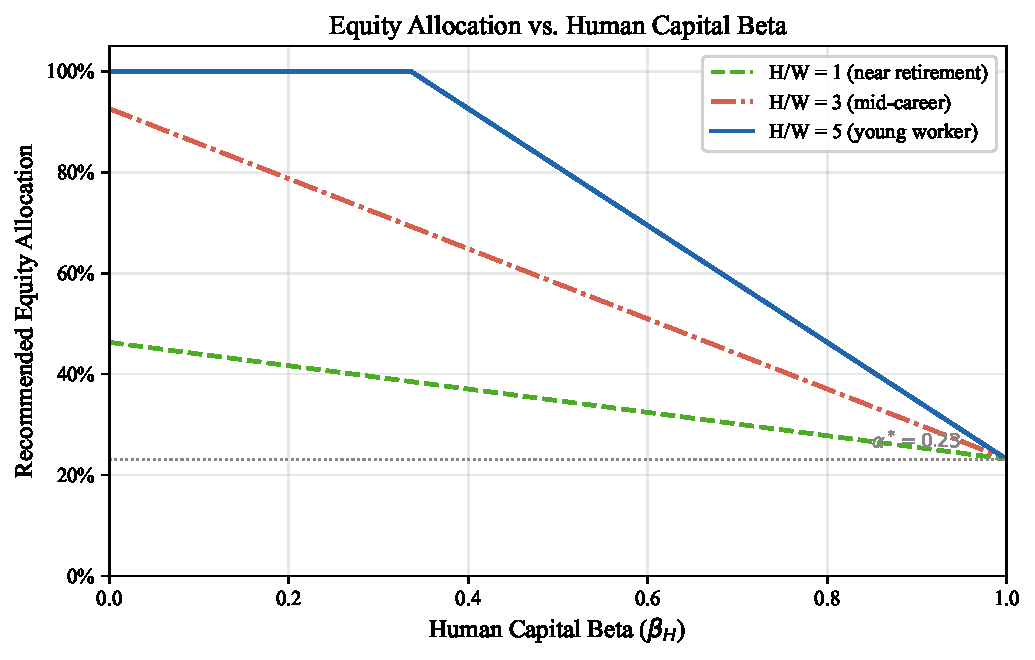
\includegraphics[width=0.85\textwidth]{figures/beta_sensitivity.pdf}
\caption{Recommended equity allocation as a function of human capital beta
($\beta_H$) for three levels of the human-capital-to-wealth ratio ($H/W$).
Market assumptions: $\mu = 0.05$, $r = 0.02$, $\sigma = 0.18$,
$\gamma = 4$. Allocations are clamped to $[0, 1]$.}
\label{fig:beta_sensitivity}
\end{figure}

\subsection{Case Studies}\label{sec:cases}

We examine three representative investors, all aged 30 with \$100{,}000 in
investable financial wealth, \$80{,}000 in annual after-tax income,
moderate risk aversion ($\gamma = 4$), and identical market assumptions
($\mu = 0.05$, $r = 0.02$, $\sigma = 0.18$). The only dimension that
differs is $\beta_H$.

\textbf{Case 1: Government employee ($\beta_H = 0$).}
This investor's income is contractually stable and uncorrelated with equity
markets. The standard model applies in full: human capital is bond-like,
and the large $H/W$ ratio justifies a high equity allocation. The
recommended allocation is at or near 100\%.

\textbf{Case 2: Technology worker with RSUs ($\beta_H = 0.60$).}
Approximately 40\% of this investor's compensation arrives as employer
RSUs. Her income is correlated with the technology sector and, by
extension, with the broad equity market. The beta-adjusted model
recognizes that 60\% of her human capital is already equity-like,
substantially reducing the diversification benefit. The recommended
allocation is approximately 30 percentage points lower than Case~1.

\textbf{Case 3: Startup founder ($\beta_H = 0.75$).}
This investor's compensation is almost entirely tied to her company's
equity value. With three-quarters of human capital behaving like equity,
the model recognizes that she is already heavily exposed to market risk
through her implicit holdings. The recommended financial portfolio
allocation is further reduced, approaching the Merton baseline
$\alpha^{*}$ with only a modest human capital uplift.

Figure~\ref{fig:balance_sheet} presents a balance sheet view comparing
Case~1 and Case~2, illustrating how the decomposition of human capital
into bond-like and equity-like components changes the effective portfolio
composition.

\begin{figure}[ht]
\centering
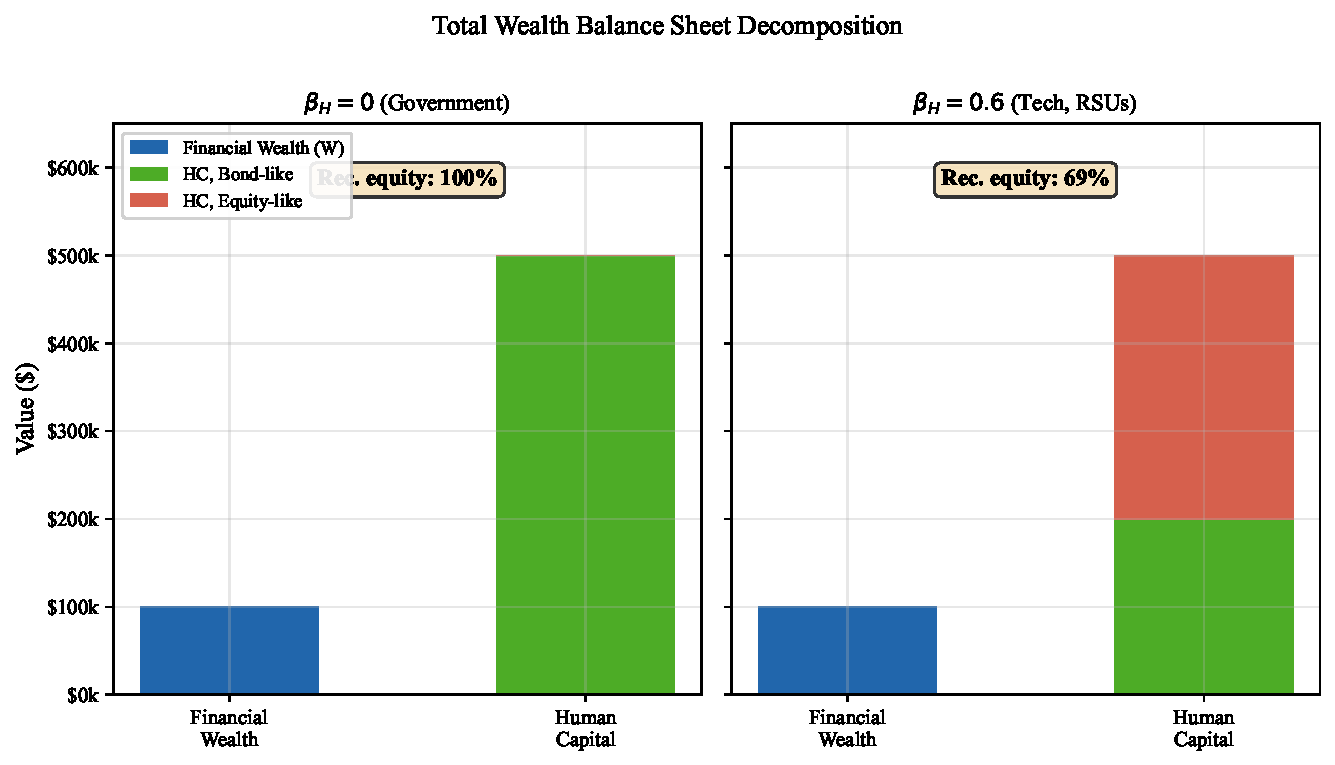
\includegraphics[width=0.85\textwidth]{figures/balance_sheet_comparison.pdf}
\caption{Total wealth balance sheet decomposition for a 30-year-old
investor with $W = \$100{,}000$ and $H = \$500{,}000$. Left panel:
$\beta_H = 0$ (government worker). Right panel: $\beta_H = 0.6$ (tech
worker with RSUs). The equity-like component of human capital (dark
shading) reduces the diversification benefit.}
\label{fig:balance_sheet}
\end{figure}

\subsection{Glide Path Implications}\label{sec:glide}

The beta-adjusted model has significant implications for lifecycle glide
paths. Figure~\ref{fig:glide} plots the recommended equity allocation
from age 25 to age 65 for three values of $\beta_H$, assuming that human
capital declines with age as the investor accumulates financial wealth and
approaches retirement.

For $\beta_H = 0$, the glide path begins near 100\% equity at age 25 and
declines to approximately 45\% by age 65, reproducing the standard
lifecycle result. For $\beta_H = 0.30$, the glide path starts lower, at
approximately 85\%, and converges to a similar endpoint. For
$\beta_H = 0.60$, the starting allocation is approximately 65\%, and the
glide path is notably flatter.

All three glide paths converge as the investor ages because $H/W$
approaches zero near retirement, making $\beta_H$ irrelevant. The
convergence is a direct consequence of equation~\eqref{eq:beta_adjusted}:
as $H/W \to 0$, the allocation approaches $\alpha^{*}$ regardless of
$\beta_H$.

\begin{figure}[ht]
\centering
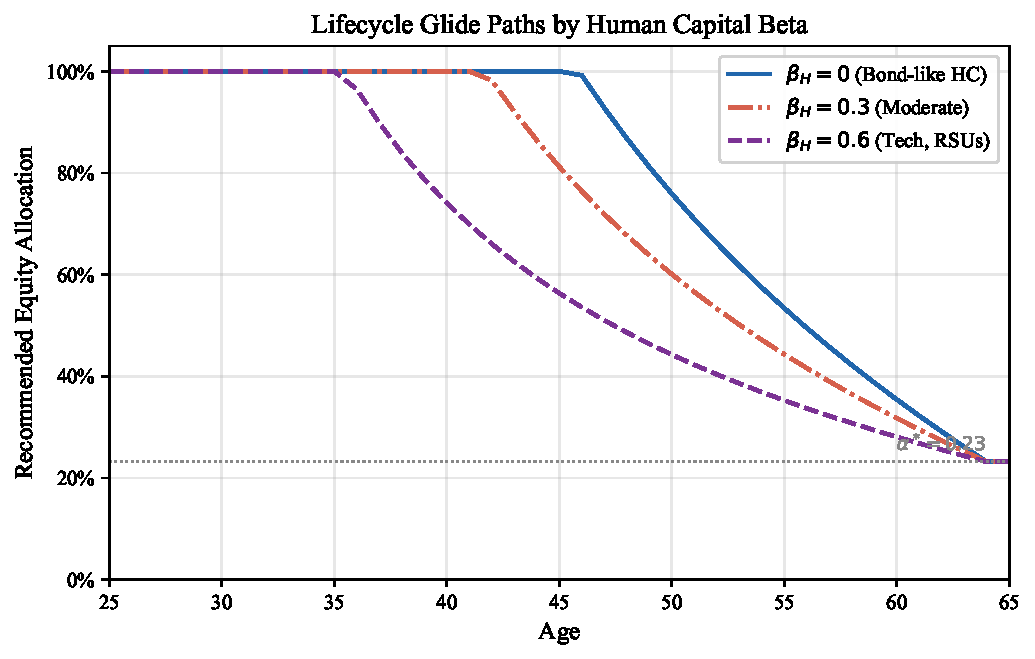
\includegraphics[width=0.85\textwidth]{figures/glide_paths.pdf}
\caption{Recommended equity allocation over the lifecycle for three levels
of human capital beta. All investors start at age 25 with
$W_0 = \$50{,}000$, income \$80{,}000, and identical market assumptions.
$H/W$ declines naturally with age as financial wealth accumulates and
remaining working years diminish.}
\label{fig:glide}
\end{figure}


% ══════════════════════════════════════════════════════════════════════
\section{Discussion}\label{sec:discussion}
% ══════════════════════════════════════════════════════════════════════

\subsection{Limitations}

Our framework involves several simplifications that warrant discussion.

\textbf{Constant beta.} We treat $\beta_H$ as constant over the
lifecycle, but in practice it may vary. A technology employee's beta
declines as RSUs vest; a startup founder's beta spikes around funding
rounds and declines after a diversifying liquidity event. Allowing
$\beta_H(t)$ to be age-dependent is a natural extension.

\textbf{Single-factor structure.} Our model assumes that the equity-like
component of human capital is correlated with the broad market portfolio.
In reality, a technology worker's income may be more correlated with the
Nasdaq than with the S\&P 500, and a real estate agent's income may track
housing prices rather than equity returns. A multi-factor extension, using
the \citet{fama1993} framework, could decompose human capital risk into
market, size, value, and industry factors.

\textbf{Idiosyncratic risk.} The parameter $\beta_H$ captures only
systematic risk. Firm-specific risk, such as a single-company RSU
concentration, creates additional uncompensated risk that is not reflected
in $\beta_H$. The practical implication is that our framework provides a
lower bound on the appropriate equity reduction: concentrated positions
warrant even lower equity allocations than $\beta_H$ alone suggests.

\textbf{Behavioral considerations.} Our model assumes rational investors
who can and will rebalance their financial portfolios. In practice, mental
accounting, inertia, and disposition effects may prevent investors from
acting on the model's recommendations.

\subsection{Extensions}

Several extensions are possible within the current framework.

\textbf{Dynamic beta.} A straightforward extension replaces the constant
$\beta_H$ with a deterministic function $\beta_H(t)$ that reflects the
changing composition of compensation over the career. For example, a
technology worker might have $\beta_H(30) = 0.60$ when RSU-heavy and
$\beta_H(55) = 0.30$ as she transitions to a more senior, cash-heavy role.

\textbf{Multi-factor model.} Replacing the single market beta with a
vector of factor betas, $\boldsymbol{\beta}_H$, allows for richer risk
decomposition. The allocation formula generalizes to account for the
investor's exposure to each factor.

\textbf{Integration with tax planning.} Workers with large RSU positions
face complex tax optimization problems around vesting, diversification,
and capital gains. Integrating the beta-adjusted framework with tax-aware
portfolio construction is a promising direction.

\subsection{Practical Implications}

For financial advisors and robo-advisory platforms, the beta-adjusted
framework provides a principled way to differentiate advice across client
segments. The key insight is operationally simple: ask about the client's
industry and compensation structure, map these to a $\beta_H$ estimate,
and apply the adjusted formula. The \texttt{lifecycle-allocation} Python
package \citep{lifecycle_allocation} provides industry beta lookup tables
and the full computation pipeline, making adoption straightforward.

For individual investors, the framework offers a useful heuristic: if a
substantial fraction of your income is tied to the stock market (through
RSUs, commissions, or cyclical employment), you should hold less equity
in your investment portfolio than standard lifecycle advice suggests. The
reduction is proportional to both the equity-like fraction of your income
and the ratio of your human capital to financial wealth.


% ══════════════════════════════════════════════════════════════════════
\section{Conclusion}\label{sec:conclusion}
% ══════════════════════════════════════════════════════════════════════

We have proposed a parsimonious extension to the lifecycle portfolio choice
framework of \citet{choi2025} that accounts for the riskiness of human
capital. The key innovation is a single parameter, the human capital beta
$\beta_H$, that captures the fraction of future earnings correlated with
equity markets. The modified allocation rule,
$\alpha = \alpha^{*}\bigl(1 + (1-\beta_H)\,H/W\bigr)$, nests the standard
bond-like human capital assumption, admits closed-form comparative statics,
and produces materially different recommendations for workers with
equity-like compensation.

Our calibration exercise reveals substantial heterogeneity across
industries, with betas ranging from zero (government, tenured education) to
0.85 (equity-heavy startup employees). For the growing population of
technology workers, finance professionals, and gig economy participants
whose income is correlated with equity markets, the standard lifecycle
model systematically overestimates the appropriate equity allocation. The
beta-adjusted framework corrects this overestimation in a theoretically
motivated and practically tractable manner.

The framework is implemented in the open-source \texttt{lifecycle-allocation}
Python library \citep{lifecycle_allocation}, available on PyPI and GitHub.
Researchers and practitioners building on this work are kindly asked to cite
both this paper and the software package.

\bigskip

% ══════════════════════════════════════════════════════════════════════
% Bibliography
% ══════════════════════════════════════════════════════════════════════
\bibliographystyle{plainnat}
\bibliography{references}

\end{document}
